\documentclass[14pt, aspectratio=169, handout]{beamer}
\usetheme{Copenhagen}
\usecolortheme{seahorse}
\setbeamertemplate{navigation symbols}{}
\setbeamertemplate{headline}{}

%\usepackage{pgfpages}
%\pgfpagesuselayout{4 on 1}[a4paper, border shrink=5mm]

\usepackage{graphicx} % Required for inserting images
\usepackage{multicol}
%\usepackage{enumitem}
\usepackage{amsfonts}
\usepackage{amsmath}
\usepackage{xcolor}

\definecolor{darkblue}{RGB}{0, 0, 139}
\definecolor{lightblue}{RGB}{173, 216, 230}

\title{SST1 Übungsstunde 2}
\author{Matteo Dietz}
\date{September 2025}

\begin{document}

\maketitle

\begin{frame}{Organisatorisches}
    \begin{itemize}
        \item \alert{Study-Center dienstags 18:15-19:00 im ETZ E7}
        \item[] Kommt in den ersten $15$ Minuten des Study-Centers!
        \item[]
        \item Vorlesungsskript und Übungsskript auf der Vorlesungswebsite
        \item[] Username: sigsys2025, \hspace{10pt} Passwort: Fourier2025
        \item[] 
        \item Link zu meinen Handouts ebenfalls auf der Vorlesungswebsite
    \end{itemize}
\end{frame}

\begin{frame}{Themenüberblick}
    \begin{itemize}
    \item \textbf{Kurze Repetition:}
    \item[] Unterräume, Normierte Lineare Räume
    \item[] 
    \item \textbf{Hilberträume:}
    \item[] Inneres Produkt, Orthogonalität, Orthonormalsysteme, $L^2$ als unendlich dimensionaler normierter Raum, Gram-Schmidt
    \item[] 
    \item \textbf{Systeme und Systemeigenschaften:}
    \item[] Linearität, Nullraum, Bildraum, Stetigkeit
\end{itemize}
\end{frame}

\begin{frame}{Aufgaben für diese Woche}
    \begin{itemize}
        \item[] \underline{\textbf{16}}, 17, \underline{\textbf{18}}, \underline{\textbf{19}}, 20, \underline{\textbf{21}}, 22, \underline{\textbf{23}}, \underline{\textbf{24}}
        \item[] 
        \item[] Die \underline{\textbf{fettgedruckten}} Übungen empfehle ich, weil sie wesentlich zu eurem Verständnis der Theorie beitragen und/oder sehr prüfungsrelevant sind.
    \end{itemize}
\end{frame}

\begin{frame}{Repetition: Lineare Unterräume}
    \begin{itemize}
        \item \textbf{Definition:} Ein linearer Unterraum ist eine \textbf{nichtleere Teilmenge} $(\Tilde{X})$ eines linearen Raumes $X$, wenn gilt:
        \item[] 
    \item[] \begin{itemize}
                \item[(i)] $x_1 + x_2 \in \Tilde{X}$, für alle $x_1, x_2 \in \Tilde{X}$.
                \item[] 
                \item[(ii)] $\alpha x \in \Tilde{X}$, für alle $\alpha \in \mathbb{C}$ und alle $x\in \Tilde{X}$.
            \end{itemize}
    \end{itemize}
\end{frame}

\begin{frame}{Repetition: Funktionsräume}

\begin{itemize}
    \item Für eine nichtleere Menge $S$ definiert man den linearen Raum $X$ als Menge aller Funktionen von $S$ nach $\mathbb{C}$, wobei die Addition und die skalare Multiplikation wie folgt definiert sind:
    \item[] 
    \item[(+)] $\forall x_1, x_2 \in X \hspace{40pt} +:X \times X \to X \hspace{12pt} $
    \item[] $(x_1 + x_2)(s) = x_1(s) + x_2(s) \hspace{8pt} \forall s \in S$
    \item[] 
    \item[($\cdot$)] $\forall \alpha \in \mathbb{C}, \; x \in X \hspace{20pt} \cdot : \mathbb{C} \times X \to X \hspace{14pt} $
    \item[] $(\alpha \cdot x)(s) = \alpha x(s)$
\end{itemize}
\end{frame}

\begin{frame}{Repetition: Normierte Lineare Räume}
    \begin{itemize}
        \item \textbf{Definition:} Ein normierter linearer Raum ist ein Paar $(X, ||\cdot||)$ bestehend aus einem linearen Raum $X$ und einer Norm auf $X$.
    \end{itemize}
\end{frame}

\begin{frame}{Hilberträume}
    \begin{itemize}
        \item Ein Hilbertraum ist ein \textbf{linearer Raum}. Dieser Raum ist
        \begin{itemize}
            \item[] 
            \item[(i)] ausgestattet mit einem \textbf{inneren Produkt}.
            \item[] 
            \item[(ii)] \textbf{vollständig} bezüglich der induzierten Norm dieses inneren Produktes.
        \end{itemize}
    \end{itemize}
\end{frame}

\begin{frame}{Vollständigkeit}
    \begin{center}
    \begin{multicols}{2}
        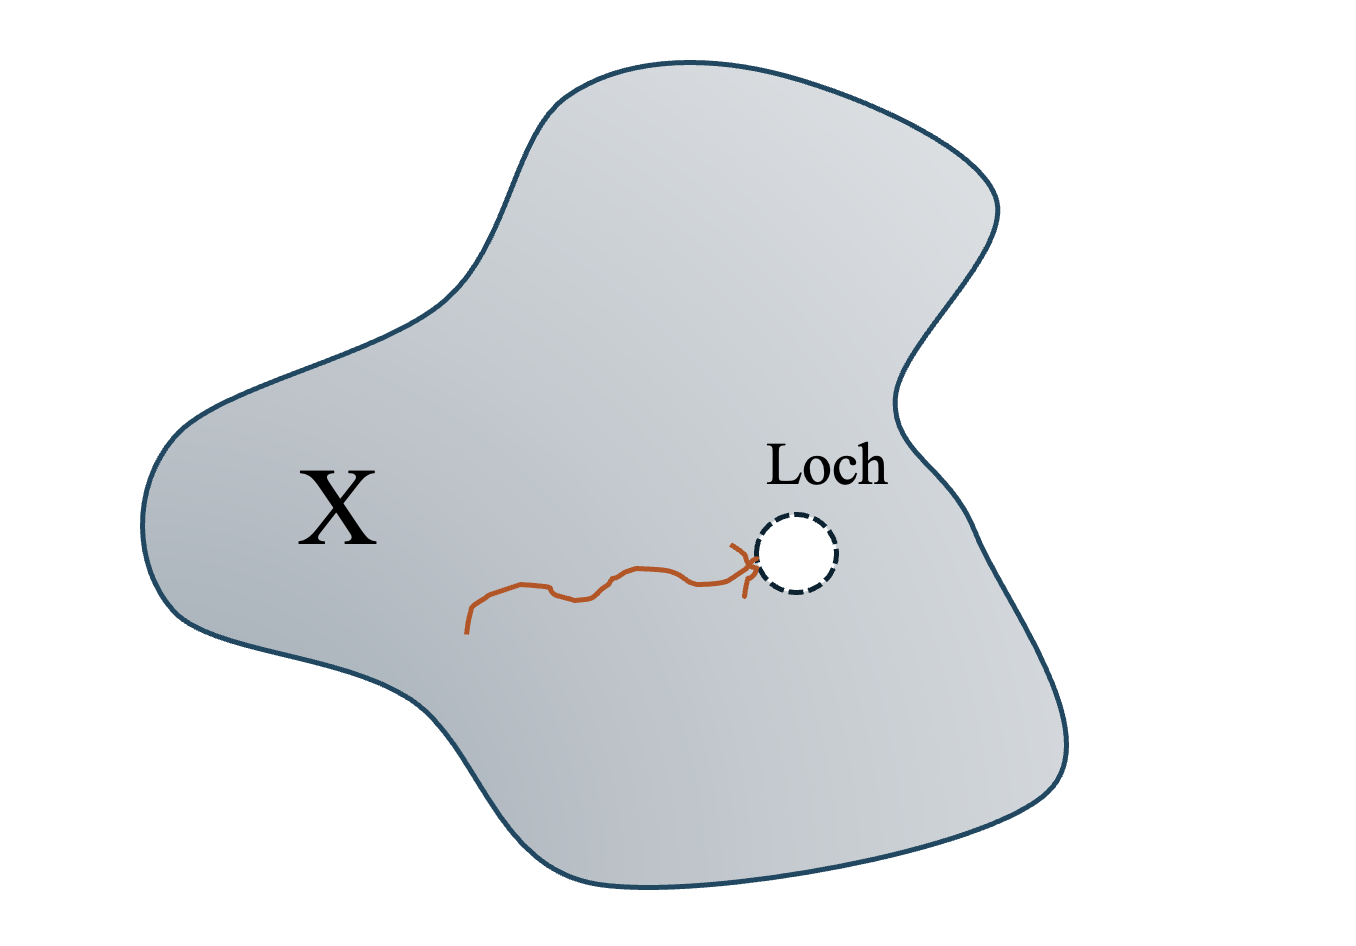
\includegraphics[width=0.7\linewidth]{figures/Kein_Hilbertraum.png}\\
        Kein Hilbertraum
        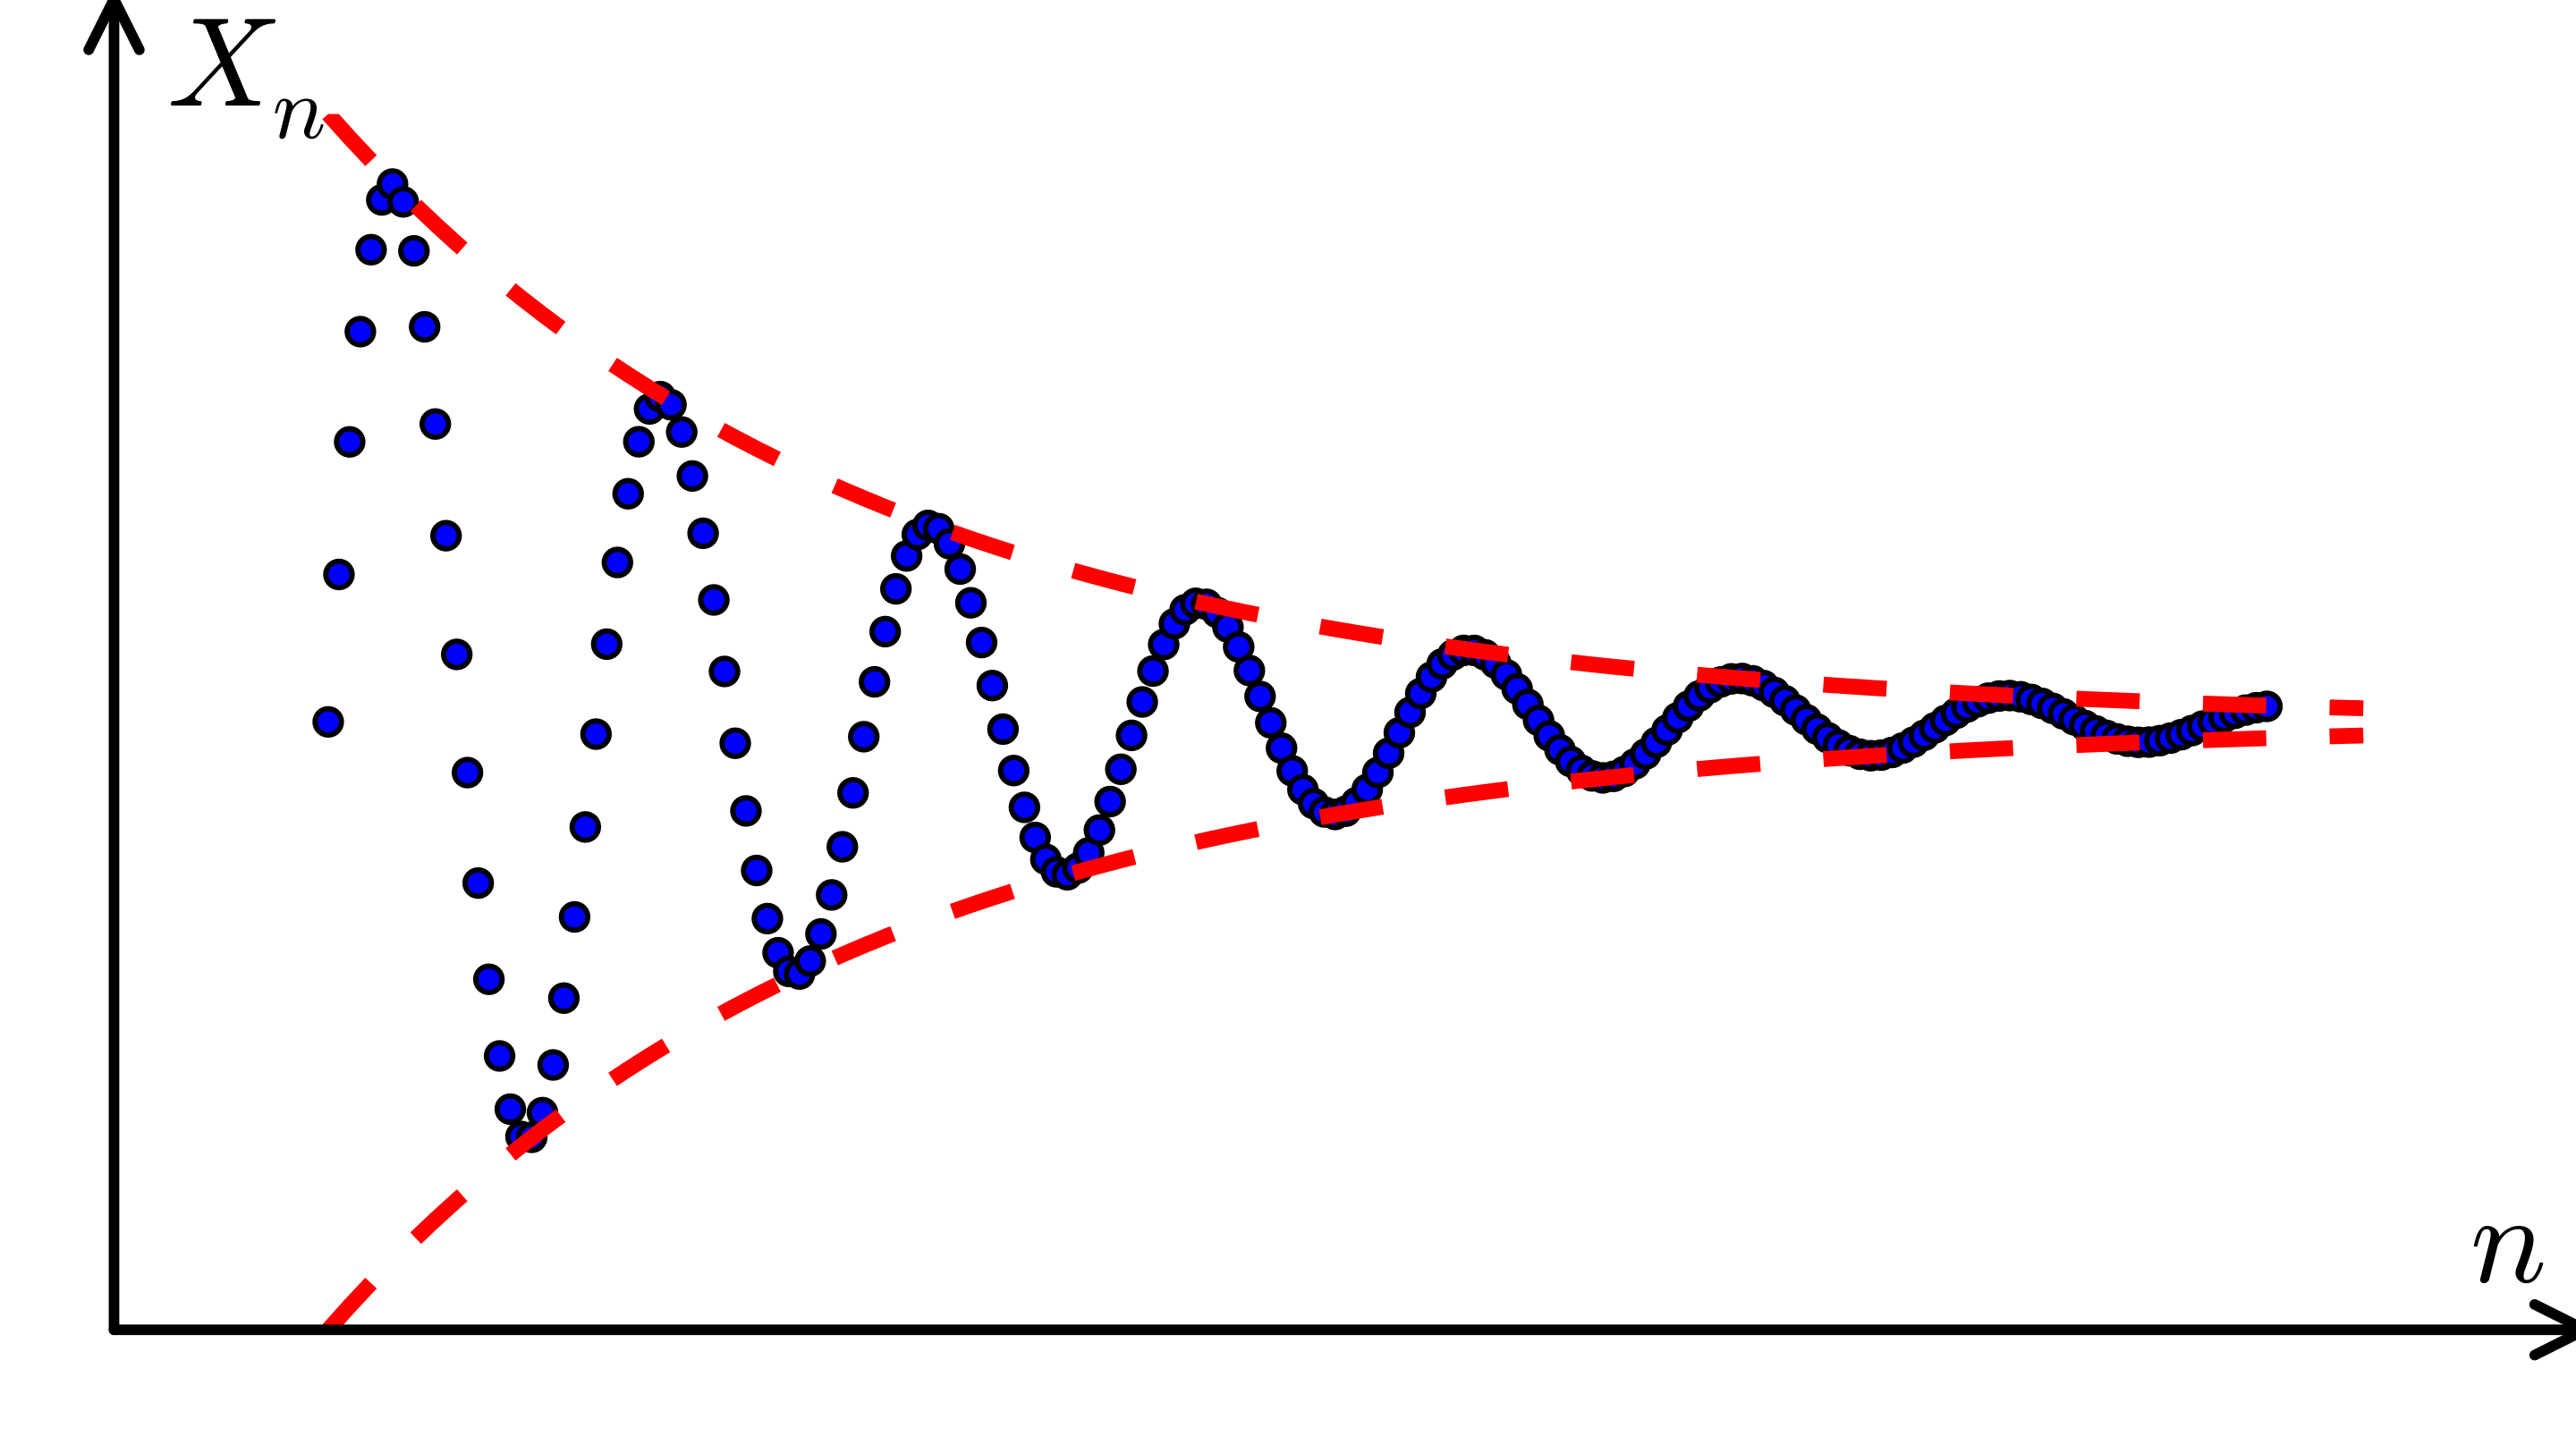
\includegraphics[width=0.9\linewidth]{figures/Cauchy_Folge.png}\\
        Cauchy-Folge
    \end{multicols}
    \end{center}
\end{frame}

\begin{frame}{Inneres Produkt: Definition}
    \begin{itemize}
        \item Die Abbildung $\langle \cdot, \cdot \rangle : X \times X \to \mathbb{C}$ in einem linearen Raum $X$ heisst \textbf{inneres Produkt}, wenn folgende Eigenschaften gelten:
            \begin{itemize}
            \item[] 
            \item[(i)] Additivität im 1. Argument: $\langle x + y, \; z\rangle = \langle x, \; z\rangle + \langle y, \; z\rangle$
            \item[] 
            \item[(ii)] Homogenität im 1. Argument: $\langle \alpha x, \; y \rangle = \alpha \langle x, \; y \rangle$
            \item[] 
            \item[(iii)] Konjugierte Symmetrie: $\langle x, \; y\rangle = \langle y, \; x\rangle^*$
            \item[] 
            \item[(iv)] Positive Definitheit: $\langle x, \; x\rangle \geq 0$ und $\langle x, \; x\rangle = 0 \Leftrightarrow x = 0$
            \end{itemize}
    \end{itemize}
\end{frame}

\begin{frame}{Inneres Produkt: Bemerkungen}
    \begin{itemize}
        \item Additiv im 2. Argument: $\langle x, \; y+z \rangle = \langle y + z, \; x \rangle^* = \langle y, \; x \rangle^* + \langle z, \; x \rangle^* = \langle x, \; y \rangle + \langle x, \; z \rangle$
        \item[] 
        \item komplexe Konjugation: $\langle x, \; \alpha y\rangle = \langle \alpha y, \; x \rangle^* = \alpha^* \langle y, \; x \rangle^* = \alpha^* \langle x, \; y \rangle$
    \end{itemize}
\end{frame}

\begin{frame}{Inneres Produkt: Induzierte Norm}
    \begin{itemize}
        \item Sei $X$ ein linearer Raum mit innerem Produkt $\langle \cdot, \cdot\rangle$
        \item[] 
        \item $||x|| := \sqrt{\langle x, \; x\rangle}$ ist die von diesem $\langle \cdot, \cdot\rangle$ \textbf{induzierte Norm}.
    \end{itemize}
\end{frame}

\begin{frame}{Orthogonalität}
    \begin{itemize}
        \item Sei $X$ ein linearer Raum mit innerem Produkt $\langle \cdot, \cdot \rangle$.
        \item[] $x_1, x_2 \in X$ sind \textbf{orthogonal}, falls $\langle x_1, \; x_2\rangle = 0$.
        \item[] 
        \item \textbf{Bemerkungen:}\begin{itemize}
            \item[(i)] Orthogonalität $\implies$ Lineare Unabhägnigkeit
            \item[] 
            \item[(ii)] $n$ paarweise orthogonale Einheitsvektoren in einem linearen Raum der Dimension $n$ bilden eine orthonormale Basis in diesem Raum.
        \end{itemize}
    \end{itemize}
\end{frame}

\begin{frame}{Satz des Pythagoras}
    \begin{itemize}
        \item[] \fcolorbox{darkblue}{lightblue}{%
        \parbox{\dimexpr\linewidth-2\fboxsep-2\fboxrule\relax}{\centering Wenn $\langle x, \; y \rangle = 0$, \hspace{10pt}dann \hspace{10pt}$||x + y||^2 = ||x||^2 + ||y||^2$}}
        \item[] 
        \item[] \textit{Beweis:} 
        \item[]
        \item[] 
    \end{itemize}
\end{frame}

\begin{frame}{Cauchy-Schwarz Ungleichung}
    \begin{itemize}
        \item[] \fcolorbox{darkblue}{lightblue}{%
        \parbox{\dimexpr\linewidth-2\fboxsep-2\fboxrule\relax}{\centering $\left|\langle u, \; v \rangle \right| \leq ||u|| \cdot ||v|| $}}
        \item[] 
        \item[] Intuition für $\mathbb{R}^2$: \hspace{10pt} $\left| \langle u, \; v \rangle \right| = ||u|| \cdot ||v|| \cdot \underbrace{\left| \cos \angle(u, \; v) \right|}_{\in [0,1]}$
    \end{itemize}
\end{frame}

\begin{frame}{Aufgabe 16}
    
\end{frame}

\begin{frame}{Vollständiges Orthonormalsystem}
    \begin{itemize}
        \item $\{e_l\}_{l = -\infty}^\infty$ in $X$ ist ein vollständiges Orthonormalsystem für den Hilbertraum $X$, wenn folgende Eigenschaften erfüllt sind:
        \begin{enumerate}
            \item[]
            \item $\langle e_l, \; e_{l'} \rangle = \begin{cases}
                1, \hspace{12pt} l = l' \\
                0, \hspace{12pt} \text{sonst}
            \end{cases}$ \hspace{12pt}, für $l,l' \in \mathbb{Z}$
            \item[] 
            \item Für jedes $x\in X$ gilt $||x||^2 = \displaystyle\sum_{l=-\infty}^\infty |\langle x, \; e_l \rangle|^2$
        \end{enumerate}
    \end{itemize}
\end{frame}

\begin{frame}{$L^2$ als unendlich dimensionaler normierter Raum}
    \begin{itemize}
        \item $L^2([0,1])$ ist der lineare Raum der auf $[0,1]$ quadratisch integrierbaren Signale. Formal:
        \item[] 
    \end{itemize}
    $$L^2\left( [0,1] \right) = \left\{ x: [0,1] \to \mathbb{C} \left| \int_0^1 |x(t)|^2 < \infty \right. \right\}$$
    \begin{itemize}
        \item $L^2([0,1])$ ist \textbf{unendlich dimensional}.
        \item[] 
        \item $\{e^{2 \pi i n t}\}_{n = -\infty}^\infty$ ist eine \textbf{ONB} in diesem Raum
    \end{itemize}
\end{frame}

\begin{frame}{$L^2$ als unendlich dimensionaler normierter Raum}
    
\end{frame}

\begin{frame}{$L^2$ als unendlich dimensionaler normierter Raum}
    
\end{frame}

\begin{frame}{Gram-Schmidt Orthogonalisierungsverfahren}
    \begin{itemize}
        \item Sei $\{ w_i \}_{i=1}^n $ eine Basis von $V$ mit Skalarprodukt $\langle \cdot, \cdot \rangle$.
        \item[] 
        \item[] Dann existiert eine \textbf{ONB} $\{v_i\}_{i=1}^n = \{v_1, \dots, v_n\}$ mit:
        \item[] 
        \item[] Span$\{v_1, \dots, v_j\} = $ Span$\{w_1, \dots, w_j\}$ für alle $j = 1, \dots, n$.
    \end{itemize}
\end{frame}

\begin{frame}{Gram-Schmidt Orthonormalisierungsverfahren}
    \fcolorbox{darkblue}{lightblue}{%
    \parbox{\dimexpr\linewidth-2\fboxsep-2\fboxrule\relax}{\begin{itemize}
    \item[] \textbf{Algorithmus}
    \item[] Für $j = 1, \; 2, \dots, n$:
    \item[] \begin{itemize}
        \item[] $v_j' = w_j - \displaystyle\sum_{i=1}^{j-1} \frac{\langle v_i, \; w_j \rangle }{\langle v_i, \; v_i \rangle} v_i$
        \item[] $v_j = \displaystyle\frac{v_j'}{||v_j'||}$
        \item[] $j \to j + 1$
    \end{itemize}
\end{itemize}}}
\end{frame}

\begin{frame}{Aufgabe 18}
    
\end{frame}

\begin{frame}{Systeme \& Beispiele}
    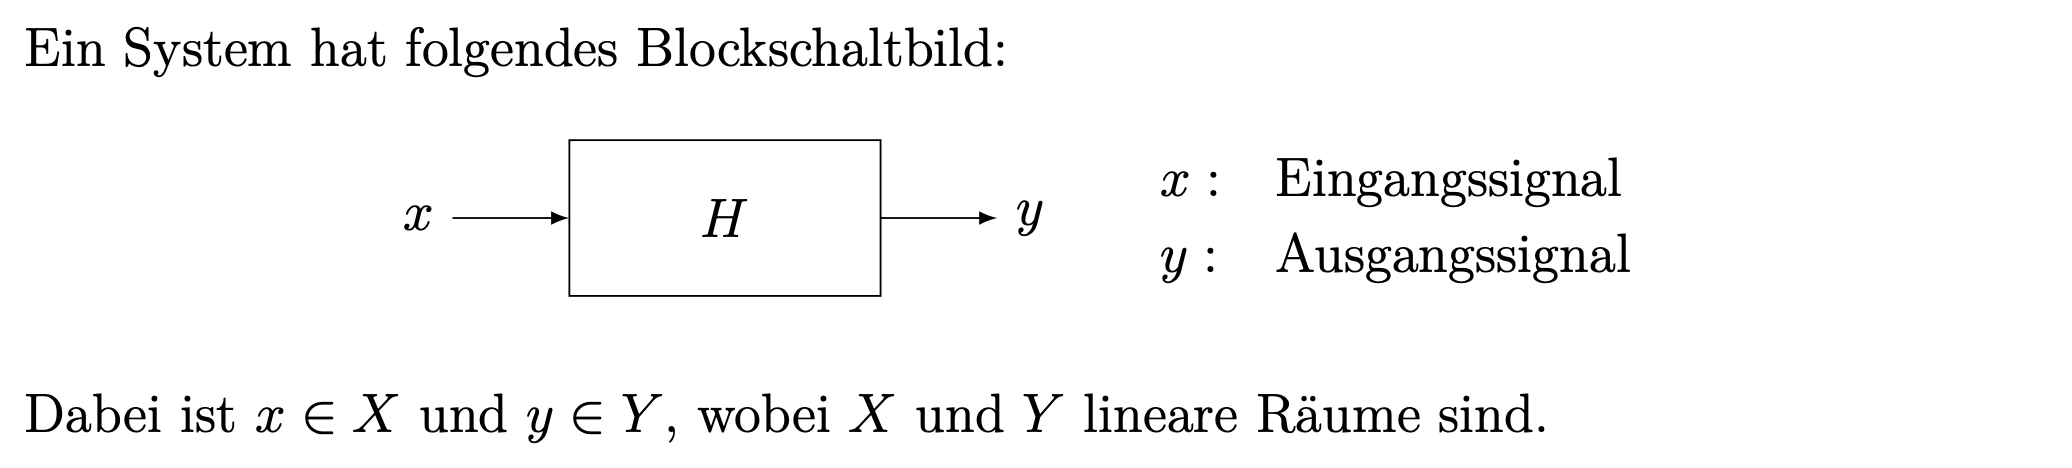
\includegraphics[width=1.1\linewidth]{figures/System_Blockschaltbild.png}
\end{frame}

\begin{frame}{Linearität}
    \begin{itemize}
        \item Ein System $H:X \to Y$ ist \textbf{linear}, wenn:
        \item[] \begin{itemize}
            \item[] 
            \item[(i)] \textbf{Additivität}: $H(x_1 + x_2) = Hx_1 + Hx_2$, für alle $x_1,x_2 \in X$
            \item[] 
            \item[(ii)] \textbf{Homogenität}: $H(\alpha x) = \alpha H x$, für alle $x\in X$ und alle $\alpha \in \mathbb{C}$
        \end{itemize}
        \item[]  
        \item Falls das System $(i) \lor (ii)$ nicht erfüllt, heisst $H$ \textbf{nichtlinear}.
    \end{itemize}  
\end{frame}

\begin{frame}{Linearität: Bemerkungen}
    \begin{itemize}
        \item Wenn $H$ ein lineares System ist, dann muss $H0 = 0$ immer gelten.
        \item[] 
        \item Wenn dies also nicht erfüllt ist, dann muss $H$ nichtlinear sein.
    \end{itemize}
\end{frame}

\begin{frame}{Aufgabe 23}
    
\end{frame}

\begin{frame}{Aufgabe 24}
    
\end{frame}

\begin{frame}{Nullraum}
    \begin{itemize}
        \item Sei $H:X \to Y$ ein lineares System
        \item[] 
        \item[] Der Nullraum von $H$ ist die Teilmenge von $X$ definiert durch $\mathcal{N}(H) = \{x \in X : Hx = 0\}$.
        \item[] 
        \item[] $\mathcal{N}(H)$ ist ein linearer Unterraum von $X$.
        \item[] 
        \item[] 
        \item[] 
    \end{itemize}
\end{frame}

\begin{frame}{Bildraum}
    \begin{itemize}
        \item Sei $H:X \to Y$ ein lineares System
        \item[] 
        \item[] Der Bildraum von $H$ ist die Teilmenge von $Y$ definiert durch $\mathcal{R}(H) = \{y =Hx : x \in X\}$.
        \item[] 
        \item[] $\mathcal{R}(H)$ ist ein linearer Unterraum von $Y$.
        \item[] 
        \item[] 
        \item[] 
    \end{itemize}
\end{frame}

\begin{frame}{Nullraum und Bildraum}
    \begin{center}
        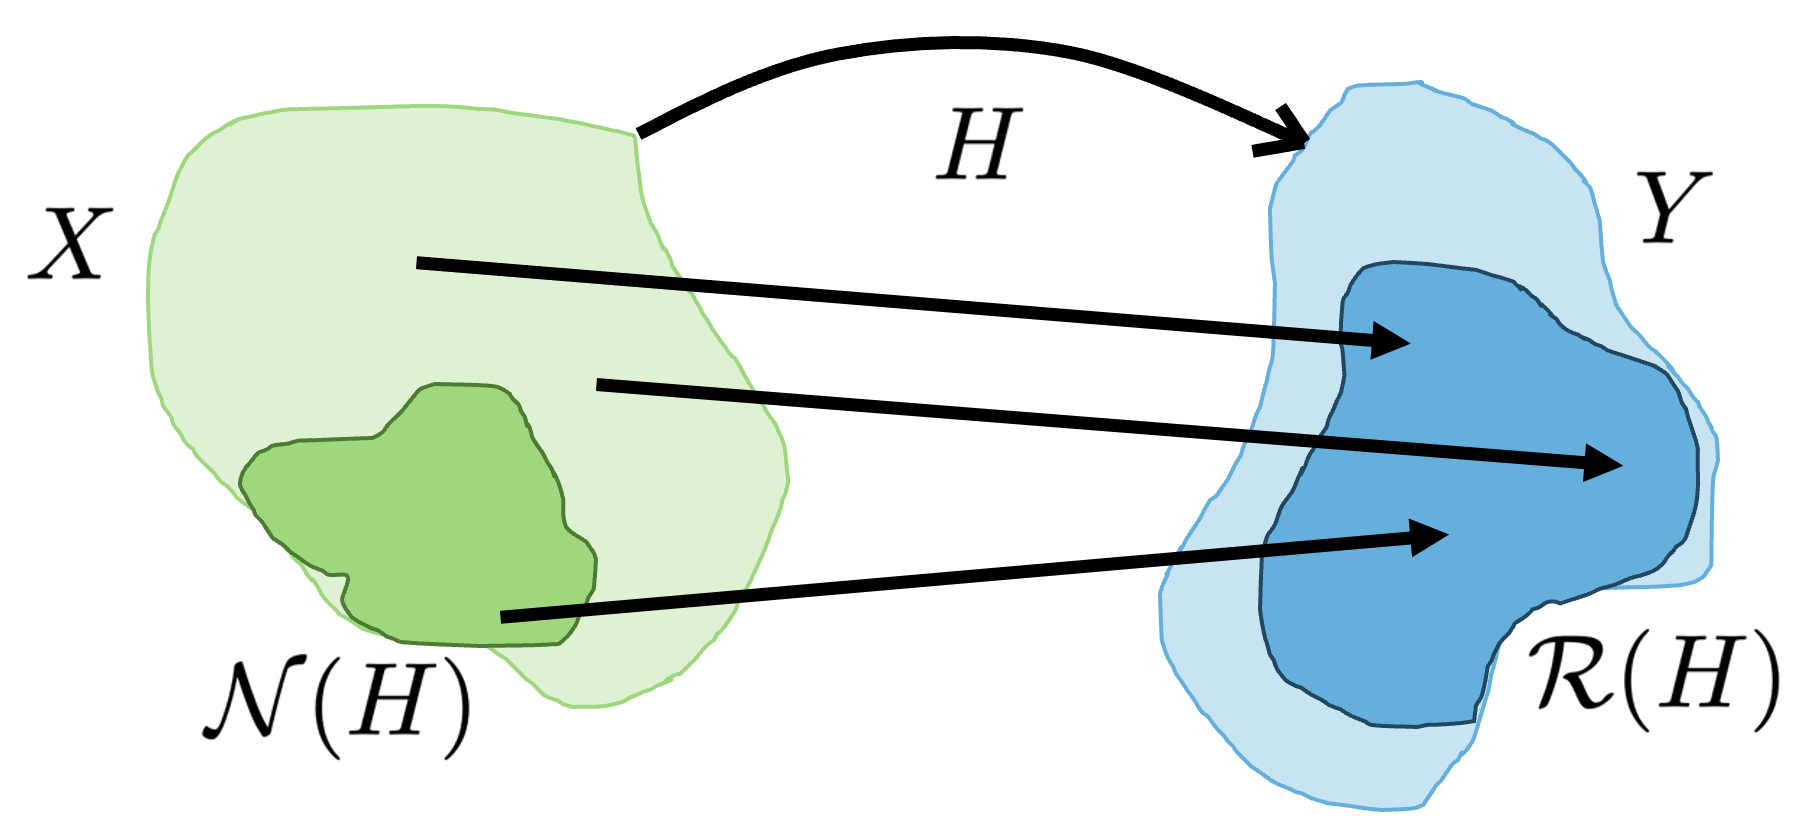
\includegraphics[width=0.9\linewidth]{figures/Bildraum_Nullraum.png}
    \end{center}
\end{frame}

\begin{frame}{Stetige Systeme}
    \begin{itemize}
        \item \textbf{Theorem:} Das System $H$ ist \textbf{linear und stetig}
        \item[] \hspace{64pt}  $\Leftrightarrow$ Für jede konvergente Reihe $\sum_{i=1}^\infty \alpha_i x_i$ gilt:
        \item[] 
    $$H\left( \sum_{i=1}^\infty \alpha_i x_i \right) = \sum_{i=1}^\infty \alpha_i H x_i$$
    \end{itemize}
\end{frame}

\begin{frame}{$\varepsilon-\delta$ Stetigkeit}
    \begin{itemize}
        \item Seien $(X, ||\cdot||))$ und $(Y, ||\cdot||))$ normierte lineare Räume.
        \item[] 
        \item[] Das System $H:X \to Y$ ist \textbf{stetig} in $x_0 \in X$, falls es zu jedem $\varepsilon > 0$ ein nur von $\varepsilon$ abhängiges $\delta >0$ gibt, so dass:
        \item[] 
        \item[] $\forall x\in X$ mit $||x-x_0||<\delta$ folgt, dass $||Hx-Hx_0||\leq \varepsilon$.
    \end{itemize}
\end{frame}

\end{document}
